%! Author = mboehme
%! Date = 23.02.2023

\subsection{Technische Umsetzung}\label{subsec:technische-umsetzung}

\subsubsection{Grobe Planung}
\newglossaryentry{deployen}{name=deployen,description={Eine Anwendung zu deployen bedeutet, sie auf einem Server zu installieren und zu konfigurieren, sodass sie für den Benutzer verfügbar ist.}}
Die Software wird als eine Azure App deployt (~\gls{deployen}).
\newglossaryentry{localhost}{name=localhost,description={Die lokale Adresse des Computers, auf dem die Anwendung läuft.}}
%glossareintrag für lokale cache cookies
Diese lässt ~\gls{localhost} Verbindungen zu und gibt einem die Möglichkeit das ganze als Single Page Application zu entwickeln, mit einem lokalen cookie cache für den eingeloggten Account.
Somit ist keine Individualisierung notwendig.
\newline
%new glossary entry for Dory-node.js
Es wird, lokal, mithilfe von Dory-node.js gehostet.
%Was ist ein phillipsdisplay
Zudem kann dann mit dem Phillips Display die Web-Applikation aufgerufen werden und als eine Art Model eines Model-View-Controllers verwendet werden.
\newline
%Das Wort "Player" einführen
Der Player benötigt auf der OMS den Content-Typen \("\)Web\("\) mit der URL: \("\)http://localhost:3000/content\("\).
Diese Seite wird dann lokal vom Player aufgerufen, worauf der Dory-node.js Server antwortet und die tatsächliche Seite anbietet, die lokal auf dem Display liegt.
%Bitte im Soll-Zustand einführen was oAuth ist
So ist die URL durchgehend, auf allen Geräten identisch, damit die OAuth 2.0 URI Bedingungen ~\cite{OAuth-2.0-Simplified} erfüllt sind.
Durch den Verzicht auf einen Webserver werden kosten eingespart, da Updates eher selten passieren sollten.
\newline
%Es gibt keinen Datenzugang
Zudem ist es für die Sicherheit der Nutzer so viel besser, da wir deshalb keinen Zugriff auf ihre Daten haben.
%Soll-Zustand - ISO 8601 Konformität
Zeiten müssen, bei jeglichen API Anfragen an die Microsoft Graph API, ISO 8601 konform sein \@.
Dies ist wichtig, da Zeitzonen des Nutzers ungleich der Zeitzonen der Server, sein können.
Außerdem können Sommer- und Winterzeiten unterschiedlich sein.
Es muss also bei der Datenverarbeitung darauf geachtet werden, dass die Zeiten immer ISO 8601 konform sind.
Bei der Anzeige müssen die Zeiten in die Zeitzone des Nutzers umrechnen.
Beispielsweise, im Terminbuchungsmenü, muss dem Nutzer die Zeit angezeigt werden, die lokal für ihn gilt.
Sobald dieser Termin aber gebucht wird, muss die Zeit in die Zeitzone des Servers umgerechnet werden, damit die Buchung auch dort korrekt verarbeitet wird.
\newline
\pagebreak
\subsubsection{Benutzte Hardware und Software}
\newline
Die Hardware ist ein Philips~\cite{10BDL4551T/00} Display.
Dieses Display ist ein 10 Zoll (ca. 25 cm) Touchscreen.
Es hat eine Auflösung von 1280x800 Pixeln und benutzt Android.
\newglossaryentry{Digital Signage}{name={Digital Signage}, description={Digital Signage ist eine Art von Werbung, die durch digitale Medien wie Displays, Fernseher oder Computer angezeigt wird.}}
Dieses Display ist für Digital Signage gedacht und kann so auch als solches verwendet werden.
\newglossaryentry{SICP}{name=SICP, description={SICP steht für Serial (Ethernet) Interface Communication Protocol.
SICP ist ein Protokoll, das es ermöglicht, mit dem Display, an der OS vorbei, zu kommunizieren.}}
Die eingebauten RGB LED Strips können per~\gls{SICP} angesteuert werden.
Dafür wird Dory-node.js genutzt, um auf einen lokalen Server zu hören und die Anfragen an das Display weiterzuleiten.
Es wird dafür keine Internetverbindung benötigt.
Dokumentationen für SICP öffentlich schwierig zu finden.
Befehle werden als Hexadezimal Werte geschrieben und an das Display gesendet.
%Quellenangabe
Die Verschlüsselung passiert, indem ein XOR aller vorausgehenden Bytes genommen und als Prüfsumme mitgegeben wird.
\newline
\newline
%In Fließtext bringen
Software:
\newline
Vue.js ist ein JavaScript Framework und transpiliert die Vue.js Dateien in JavaScript, damit sie von jedem Browser ausgeführt werden können.
Es ist darauf spezialisiert, Single Page Applikationen zu entwickeln.
\newline
\newline
\newglossaryentry{Node.js Server}{name={Node.js Server}, description={Ein Node.js Server ist ein Server, der auf Node.js basiert und JavaScript Code ausführt.}}
Dory-Node.js ist ein Node.js Server, der es ermöglicht, eine Web-Applikation lokal zu hosten.
Dies wird benötigt, um einerseits die Raumbuchungsseite lokal anzubieten, damit die absoluten Redirect-URI Bedingungen von Microsoft und oAuth 2.0 erfüllt werden können und andererseits, um die Anwendung auf dem Display zu hosten und als Schnittstelle zwischen der Seite und dem den LED-Strips des Displays zu agieren.
\newline
\newline
\newglossaryentry{NPM}{name=NPM, description={NPM steht für Node Package Manager.}}
Die Microsoft Graph API wird per ~\gls{NPM} Package verwendet, um die Anfragen an die Microsoft Graph API zu vereinfachen und den User einzuloggen.
\newline
\newline
Babel ist ein JavaScript Compiler, der es ermöglicht, moderne JavaScript Features zu verwenden, die von älteren Browsern nicht unterstützt werden, um so die Kompatibilität zu erhöhen.
\newline
\newline
Webpack ist ein JavaScript Bundler, der es ermöglicht, mehrere JavaScript Dateien zu einer einzigen zusammenzufassen, um so die Ladezeiten zu verkürzen.
\newline
\newline
Node.js ist ein JavaScript Runtime, der es ermöglicht, JavaScript Code auszuführen, ohne einen Browser zu benötigen.
Es ist das Backend dieser Anwendung.
Dieser wird per Dory-Node.js gehostet.
\newline
\newline
Git ist ein dezentrales Versionskontrollsystem, welches es ermöglicht, Änderungen an Dateien zu verfolgen und zu verwalten.
Dies wurde in Zusammenhang mit GitLab verwendet, da dies der derzeitige, etablierte Standard der DooH media GmbH ist.
\newline
\newline
\newglossaryentry{Linter}{name=Linter, description={Ein Linter ist ein Programm, das es ermöglicht, Code auf Fehler zu prüfen.}}
EsLint ist ein ~\gls{Linter}, der es ermöglicht, JavaScript Code zu analysieren und zu formatieren.
Da Testfälle bei JavaScript Projekten nicht immer vollständig möglich sind, ist es wichtig, dass der Code einheitlich ist und keine syntaktischen Fehler enthält.
Deshalb achtet EsLint auf die Einhaltung von Regeln, damit erst gar keine Fehler entstehen, die der JavaScript Compiler nicht erkennen kann.
Beispielsweise wird überprüft, ob Variablen deklariert wurden, bevor sie verwendet werden und anders herum.
\newline
\newline
IntelliJ IDEA ist eine IDE, die es unter anderem ermöglicht, JavaScript Code zu schreiben und zu debuggen.
\newline
\newline
%Entwicklung fängt schon vorher an.
\subsubsection{Weiterentwicklung der groben Planung}
Es wurde eine Azure App erstellt, die die Authentifizierung der Anwendung und des Benutzers übernimmt.
\newline
Dort wird der Benutzer eingeloggt und die Anwendung leitet ihn auf die Seite weiter, die er vorher besucht hat, welche in diesem Fall, die Raumbuchungsseite ist.
\newline
Es wurde jede Woche Rücksprache mit dem Kunden gehalten, um die Anforderungen zu besprechen und zu erfüllen.
Aber auch intern wurde Rücksprache gehalten, was denn sinnvoll ist und was nicht.
\newline
%Iterative Entwicklung mit Kundenentwicklung. Vllt eigenes Kapitel
So wurde jede Woche die Anwendung weiterentwickelt und verbessert.
Teilweise wurden auch neue Features hinzugefügt, die nicht initial erwünscht, aber sinnvoll waren.
Manche Features wurden auch wieder entfernt, da sie nicht sinnvoll waren oder von anderen Features abgedeckt wurden.
\newline
%Ablauf der Entwicklung
\newline
\subsubsection{Ablauf der Entwicklung}
Nachdem der erste Prototyp fertig war und Rücksprache gehalten wurde, wurde angefangen die Anwendung zu entwickeln.
Design und Funktionalität wurden dabei partiell parallel entwickelt, wobei die Funktionalität immer Priorität hatte.
In über 95 Commits wurden die Änderungen an der Anwendung festgehalten.
\newline
Es wurde ein Testgerät benötigt, um die Anwendung zu testen.
Ein Phillips 10BDL4551T/00 Display wurde dafür an die Wand gehängt und mit dem Internet verbunden.
%Warum mit Internet verbunden?
Zudem wurde es so eingerichtet, wie es auch beim Kunden laufen soll.
\newline
Es wurde täglich aktiv genutzt, um so Fehler zu finden und Feedback zu geben.
Das Feedback wurde dann evaluiert.
Solche explorativen Tests sind sehr wichtig, um Intuitivität und Benutzerfreundlichkeit zu gewährleisten.
Es war einerseits hilfreich, um vorgesehene Abläufe zu testen, andererseits aber auch um Fehler zu finden, die nicht vorgesehen waren, indem Monkey Testing~\cite{Monkey-Testing-Book1} betrieben wurde.
\newline
\subsubsection{Rest-Anfragen}
Mithilfe der oDatav4 (~\cite{oData}) API wurden die Daten aus der jeweiligen Microsoft Datenbank im Voraus gefiltert, um so nicht notwendige Daten zu vermeiden und die Performance drastisch zu erhöhen, als auch Datenvolumen zu sparen.
Die Daten wurden dabei im JSON Format zurückgegeben.
Die oData v4 API verhält sich dabei wie eine SQL Datenbank, wobei die Daten in Tabellen gespeichert sind.
%Satz zu lang, umformieren
Es wurden die Klauseln \("\$\)filter\("\) und \("\$\)top\("\) verwendet, um nur Termine für den aktuellen und nächsten Tag zu erhalten und dies einzuschränken auf die top 300 Termine, falls jemand versucht das System zu überlasten.
Eine Sortierung ist nicht notwendig, da die Termine bereits nach Startzeit sortiert sind.
Hier sieht man die oData v4 API Anfrage:
\newline
%add Fix code listing and remove .
\begin{lstlisting}[language=javascript,label={lst:JavaScript oData v4 API Anfrage}]
     let url =  "https://graph.microsoft.com/v1.0/me/findMeetingTimes/?$filter=start/dateTime" +  "ge"  + "${todayDate} and end/dateTime le ${tomorrowDate}&$top=300";
\end{lstlisting}
%Anfrage erläutern
\newline
%Probleme gehören eigentlich woanders hin
Es wurden im Voraus Befehle im Microsoft Graph Explorer~\cite{Microsoft-Graph-Explorer} ausgeführt, um zu testen, ob die Anfrage funktioniert und ob die Daten in der gewünschten Form zurückgegeben werden.
Jedoch hat sich herausgestellt, dass der Microsoft Graph Explorer nicht korrekt funktioniert und teilweise Befehle nicht entgegennimmt, die laut Microsoft Dokumentation funktionieren sollten.
Evident ist dies, da die Anwendung korrekt funktioniert und die REST API Anfragen korrekt funktionieren und auch im Request-Response Zyklus keine Fehler auftreten.
\newline
\newline
Falls die Anfrage nicht funktioniert, wird eine Fehlermeldung angezeigt, die den User darauf hinweist, dass die Verbindung zum Server derzeit unterbrochen ist.
%Soll-Zustand
Fehlermeldungen sollten immer so gestaltet sein, dass sie den User nicht verunsichern (~\cite{interaction-design-book1}), sondern ihn auf die Lösung des Problems hinweisen.
Auch bei der Gestaltung der Fehlermeldung sollte darauf geachtet werden, dass sie nicht zu lang ist, da der User sonst nicht mehr weiß, was er tun soll.
Bei Kiosk Anwendungen ist es besonders wichtig, dass die Fehlermeldungen kurz und prägnant sind, da der User ohnehin in einer Situation ist, in der er wahrscheinlich nicht viel Zeit hat.
%Genaueres dazu, befindet sich, im genannten Buch, unter dem Kapitel \("Errors, Alerts, and Confirmation"\) und unter dem Kapitel \("Platform and Posture - Designing for kiosks"\).
Das bedeutet, dass Fehler, die dazu führen, dass die Anwendung nicht mehr funktioniert, groß und auffällig dargestellt werden sollten, damit der User sie nicht übersehen kann und versteht, dass er die Anwendung nicht mehr nutzen kann, bis das Problem behoben wurde.
Andererseits sollten Fehler, die nicht dazu führen, dass die Anwendung nicht mehr funktioniert, klein und unauffällig dargestellt werden, damit der User nicht gestört wird.
\newline
\newline
Hier sieht man ein Sequenzdiagramm, welches die Kommunikation zwischen der Anwender und dem Server darstellt:
\newline
\newline
\par\vspace{0.5cm}
\centering
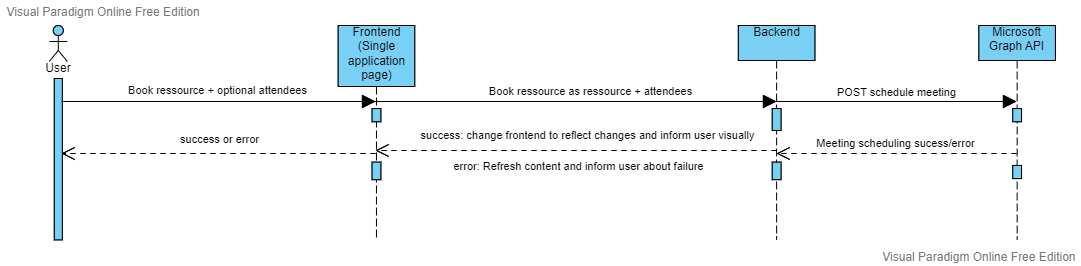
\includegraphics[width=\textwidth]{Bilder/Objektorientiertes Design/Sequence diagram for ressource booking (3)}
\par\vspace{0.5cm}
\raggedright
\newline
\newline
%Soll-Zustand einführen
\subsubsection{Timer}
Der Timer, welcher die übrig bleibende Zeit bis zum Ende des jetzigen Termins anzeigt funktioniert, wie folgt:
\newline
\newline
Es wird die Zeit bis zum Ende den jetzigen Termin berechnet, ausgehend von der Zeit, die zum Anfang des jetzigen Termins vergangen ist, und in Millisekunden umgerechnet.
Dann wird eine sich drehende Animation erstellt, die für diese Dauer abläuft.
\newline
Da die Dauer angepasst werden kann, muss bei Datenänderungen geprüft werden, ob sich die Dauer verändert hat.
%Glossar local storage
Die Daten dafür werden im Local Storage gespeichert.
Falls eine Änderung stattgefunden hat, wird die Animation neu berechnet.
Bei der Änderung werden, damit die Animation visuell nicht von vorne anfängt, die Animationsdauer und die vergangene Zeit als neue Animationsdauer aufaddiert und die vergangene Zeit als negative Animationsverzögerung gesetzt, damit die Animation visuell betrachtet dort ist, wo sie relativ zur neuen Dauer sein sollte.
\newline
\newline
Die Formel lautet, wie folgt:
\newline
\newline
\begin{equation}
\begin{aligned}
    \text{Vergangene Zeit} &= \text{Jetzt} - \text{Start} \\
\text{Animationsdauer} &= \text{Ende} - \text{Start} \\
    \text {Animationsverzögerung} &= \text{-Vergangene Zeit} \\
\end{aligned}
\end{equation}
\newline
\newline
Die Berechnung wurde wie folgt implementiert:
\newline
\newline
\begin{lstlisting}[language=javascript,label={lst:JavaScript Timer}]
let currentEventBeginningTime = localStorage.getItem('currentEventBeginningTime');
let timePassed = (new Date() - new Date(currentEventBeginningTime + 'Z')) / 1000;
let animationDuration = ((new Date(currentEventEndTime + 'Z') - new Date(currentEventBeginningTime + 'Z')) / 1000);
firstHandSpan.style.animationDuration = animationDuration  + 's';
secondHandSpan.style.animationDuration = animationDuration + 's';
firstHandSpan.style.animationDelay = -timePassed + 's';
secondHandSpan.style.animationDelay = -timePassed  + 's';
\end{lstlisting}
\newline
\newline
Um die Animation während ihrer Laufzeit zu ändern, wird ein sogenannter Reflow ~\footcite{JavaScriptAnimationsReflow} erzwungen, indem die offsetWidth Eigenschaft abgefragt, die Animationsdauer und -verzögerung neu gesetzt und der Animationsname erst entfernt und dann wieder hinzugefügt wird.
\newline
\newline
\subsubsection{Persistente Datenspeicherung}
Um die Daten der Anwendung zu speichern, wurde für kleinere Datensätze der Local Storage verwendet.
Dieser ist in jedem Browser verfügbar und darf bis zu 5 MB groß sein.
\newline
\newline
Für größere Datensätze wurde IndexedDB~\cite{IndexedDB} verwendet.
\newglossaryentry{caniuse}{name={caniuse.com},description={Caniuse is a website that shows you browser support for various features and includes references to the relevant specifications.}}
Dies ist eine NoSQL Datenbank, die in jedem gängigen Browser~\cite{caniuse-indexedDB} (\gls{caniuse}) verfügbar ist.
Die maximale Größe bei Chrome beträgt 80\(\%\) des verfügbaren Speichers.
Da es im Internet viele, sich widersprechende Angaben zu dieser Größe gibt, wurde diese manuell, mit folgendem Code, in der Konsole des Browsers, getestet:
\newline
\newline
\begin{lstlisting}[language=javascript,label={lst:JavaScript IndexedDB Speichergröße}]
    if (navigator.storage && navigator.storage.estimate) {
    const quota = await navigator.storage.estimate();
    // quota.usage -> Number of bytes used.
    // quota.quota -> Maximum number of bytes available.
    const percentageUsed = (quota.usage / quota.quota) * 100;
    console.log("You've used ${percentageUsed}% of the available storage.");
    const remaining = quota.quota - quota.usage;
    console.log("You can write up to ${remaining} more bytes.");
    }
\end{lstlisting}
\newline
\newline
Die Festplatte, auf der dies getestet wurde, hatte ca. 828 GB freien Speicher.
Das Ergebnis lautete, wie folgt:
\newline
\newline
\begin{lstlisting}[language=javascript,label={lst:JavaScript IndexedDB Speichergröße Ergebnis}]
    You've used 0.000002393592594674544% of the available storage.
    You can write up to 599726105785 more bytes.
\end{lstlisting}
\newline
\newline
%equation
\begin{equation}
    \begin{aligned}
       \text{verbleibender Speicher} &= \text{599726105785 Bytes}\\
       \newline
       \text{599726105785 Bytes} \text{ * 10}\textsuperscript{-9} &= \text{599,726105785 Gigabytes}\\
        \newline
        \newline
    \end{aligned}
\end{equation}
\newline
\newline
Das sind etwas über 70 \%\) der verfügbaren Speicherkapazität.
Hier ist davon auszugehen, dass die restlichen 10 \%\) für andere Daten schon verwendet werden.
Zudem ist zu betrachten, dass die \"\).\"\) Schreibweise für Dezimalzahlen in JavaScript verwendet wurde, während wiederum die \"\),\"\) Schreibweise für die mathematische Gleichung verwendet wurde.
Dies hat den Hintergrund, dass die \"\),\"\) Schreibweise in JavaScript nicht grundsätzlich unterstützt wird, beziehungsweise, die Konvention beim Programmieren verlangt, dass man auf Englisch programmiert und im Englischen die Dezimalzahlen mit einem Punkt geschrieben werden.
\newline
\newline
Die Datenbank befindet sich aufgrund ihrer geringen Komplexität in der 5. Normalform.
Der Schlüssel besteht aus dem Namen der Firma, zu der, das Logo gehört und gibt das nicht Primärattribut zurück, welches das Bild, in Base64, enthält.
Schlüssel müssen eindeutig sein.
IndexedDB unterstützt die Eigenschaft \"\)unique\"\), welche dafür sorgt, dass der Schlüssel eindeutig ist.
Jedoch gehen wir auch manuell noch einmal sicher, dass der Schlüssel eindeutig ist, also dass sich dieser, noch nicht in der Datenbank befindet.
Eine weitere Aufteilung würde zu Informationsverlust führen, da der Firmenname eindeutig ist.
\newline
\newline
Zwar gibt es die Möglichkeit die Bilder für Firmen, zu updaten, welcher der User auch so wahrnimmt, jedoch wird der Schlüssel des alten Bildes entfernt und ein neuer Schlüssel mit dem neuen Bild hinzugefügt.
Dies ist notwendig, da der Schlüssel eindeutig sein muss.
Somit löschen wir den alten Eintrag und fügen einen neuen hinzu.
Unabhängig von der Interaktion mit der Datenbank, wird sichergestellt, dass sinnfreie Anfragen an die Datenbank nicht gesendet werden.
Falls der User beispielsweise ein Bild hochlädt, welches bereits in der Datenbank, für genau den gleichen Schlüssel, vorhanden ist, wird die Anfrage an die Datenbank nicht gesendet oder falls der User versucht ein Bild aus der Datenbank zu entfernen, welches gar nicht existiert.
\newline
\newline
%Tabelle erläutern
\subsubsection{Azure Authentifizierung}\label{subsubsec:Azure Authentifizierung}
Um die Authentifizierung zu realisieren, wurden folgende Berechtigungen benötigt:
\newline
\newline
%    \begin{table}
    \centering
%table should not be wider than 0.8\textwidth
\small
    \begin{tabularx}{\textwidth}{|X|X|X|}
        \toprule
        \textbf{Calendars.Read} & \textbf{Delegiert} & \textbf{Lesezugriff auf Benutzerkalender}\\
        \midrule
        Calendars.Read.Shared & Delegiert & Benutzer und freigegebene Kalender lesen\\
        Calendars.ReadWrite & Delegiert & Verfügt über Vollzugriff auf Benutzerkalender.\\
        Calendars.ReadWrite.Shared & Delegiert & Benutzerdefinierte und freigegebene Kalender lesen und schreiben\\
        email & Delegiert & E-Mail-Adresse von Benutzern anzeigen \\
        IMAP.AccessAsUser.All & Delegiert & Read and write access to mailboxes via IMAP.\\
        Mail.Read & Delegiert & Lesezugriff auf Benutzer-E-Mails\\
        Mail.Send & Delegiert & E-Mails unter einem anderen Benutzernamen senden\\
        Mail.Send.Shared & Delegiert & E-Mails im Namen anderer Benutzer senden\\
        offline\_access & Delegiert & Zugriff auf Daten beibehalten, für die Sie Zugriff erteilt haben\\
        OnlineMeetings.Read & Delegiert & Read user's online meetings\\
        OnlineMeetings.ReadWrite & Delegiert & Read and create user's online meetings\\
        openid & Delegiert & Benutzer anmelden\\
        profile & Delegiert & Grundlegendes Profil von Benutzern anzeigen\\
        User.Read & Delegiert & Anmelden und Benutzerprofil lesen\\
        \bottomrule
    \end{tabularx}
    \caption{}
    \label{tab:}
%    \end{table}
\newline
\newline
\raggedright
\normalsize
Diese werden beim erstmaligen Login, vom User, seitens Microsoft, angefordert.
Ohne die Zustimmung des Users, wird die Anwendung nicht entsprechend den Anforderungen, funktionieren und wird weiterhin darauf hinweisen, dass der User sich anmelden soll.
